\begin{wrapfigure}{l}{0.95\textwidth}
  \vspace{-6pt}
  \scalebox{0.9}{
    \hspace{-8pt}
    \begin{tabular}{m{1pt}cc}
      \raisebox{110pt}{
      \rotatebox{90}{magnitude $w_i$}
      }
      &
      \hspace{8pt}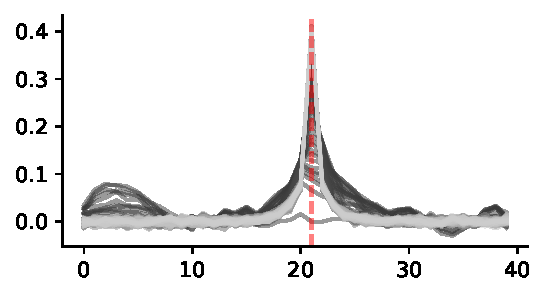
\includegraphics[width=0.5\linewidth]{figures/peak-failure/ising.pdf}
      &
      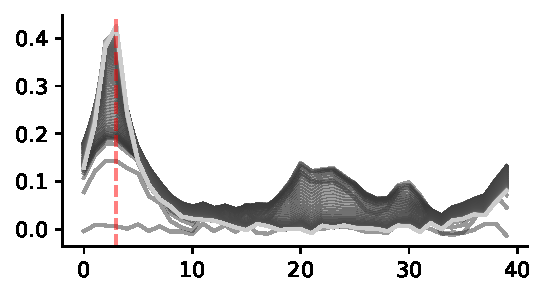
\includegraphics[width=0.5\linewidth]{figures/peak-failure/ising_kurtosis.pdf}  \\
      \noalign{\vskip -84pt}
      & 
      \hspace{22pt}
      dimension $i$ of weight $\mathbf{w}$ & 
      \hspace{22pt}
      dimension $i$ of weight $\mathbf{w}$ 
    \end{tabular}
  }
  \caption{
    Failure case for peak prediction, as discussed in \cref{sec:peak-prediction}.
    The (\textbf{left}) simulated receptive field localizes with a peak at index $i=21$, while the (\textbf{right}) integrated receptive field localizes at $i=3$.
    This is because localization is extremely sensitive to initial conditions in the weights $\mathbf{w}$.
    This sensitivity manifests as a second bump near $i=3$ for the simulated receptive field earlier in training (darker lines).
    In the integrated receptive field, there is a large bump near $i=21$ early in training, which corresponds to the true peak location.
    Thus, our approximation in integrating identifies these competing bumps, but predicts the wrong one wins out.
  }
  \label{fig:peak-failure}
\end{wrapfigure}
